\documentclass[a4paper]{article}
\usepackage{xcolor}
\usepackage{hyperref}
\usepackage[tightLists=false,hybrid=true]{markdown}
\usepackage[utf8]{inputenc}
\usepackage[T1]{fontenc}
\usepackage{hyperref} % Required for adding links	and customizing them
\definecolor{linkcolour}{rgb}{0,0.2,0.6} % Link color
\hypersetup{colorlinks,breaklinks,urlcolor=linkcolour,linkcolor=linkcolour} % Set link colors throughout the document
\urlstyle{rm}


\usepackage[sc]{titlesec}
\titleformat{\section}{\Large\bfseries\sc\centering}{\thesection}{0em}{}
\titleformat{\subsection}{\Large\bfseries\sc\raggedright}{}{1em}{}
%\renewcommand{\thesubsection}{}
%\renewcommand{\thesection}{\arabic{section}}

\title{\textsc{\LARGE 2018 Work Log}\\ }
\date{}


\begin{document}
\maketitle


\section*{January}

\begin{markdown}
## Week 1

Returned from vacation in s.e. asia on Monday. I started working with easy maintenance tasks on my code.

- Created a git `development` to keep the `master` branch stable at all times.
- Polished up the `cmake` build script so that libraries are either found or fetched and installed properly in a platform independent way. Took some trial and error. 
- Added support for \href{www.travis-ci.com}{Travis-CI}, so that a `git push` now triggers a build in `g++-7.2` and `clang++-5.0`, and reports pass/fail on the github page.
- Added support for reading parameters from a text file instead of hard-coding them into a namespace .
- Rewrite routines for finding files in the filesystem, making better use of `<std::experimental::filesystem>` features for finding input and output files.

## Week 2

Continued on maintenance work. Almost finished

- Fixed some profiling issues. Timings were not clear enough.
- Fixed console output and implemented optional verbosity level, and optional timestamps.
- Started restructoring the algorithms using smart pointers everywhere, and using a Base class from which algorithms are derived (itebd, idmrg, fdmrg, etc). This modularization will speed up development time later, I believe.

## Week 3

- 


## Week 4
This week I started a new project: excited-state DMRG. I am supposed to implement SIMPS or xDMRG and then study the MBL transition shown in the picture.

\centering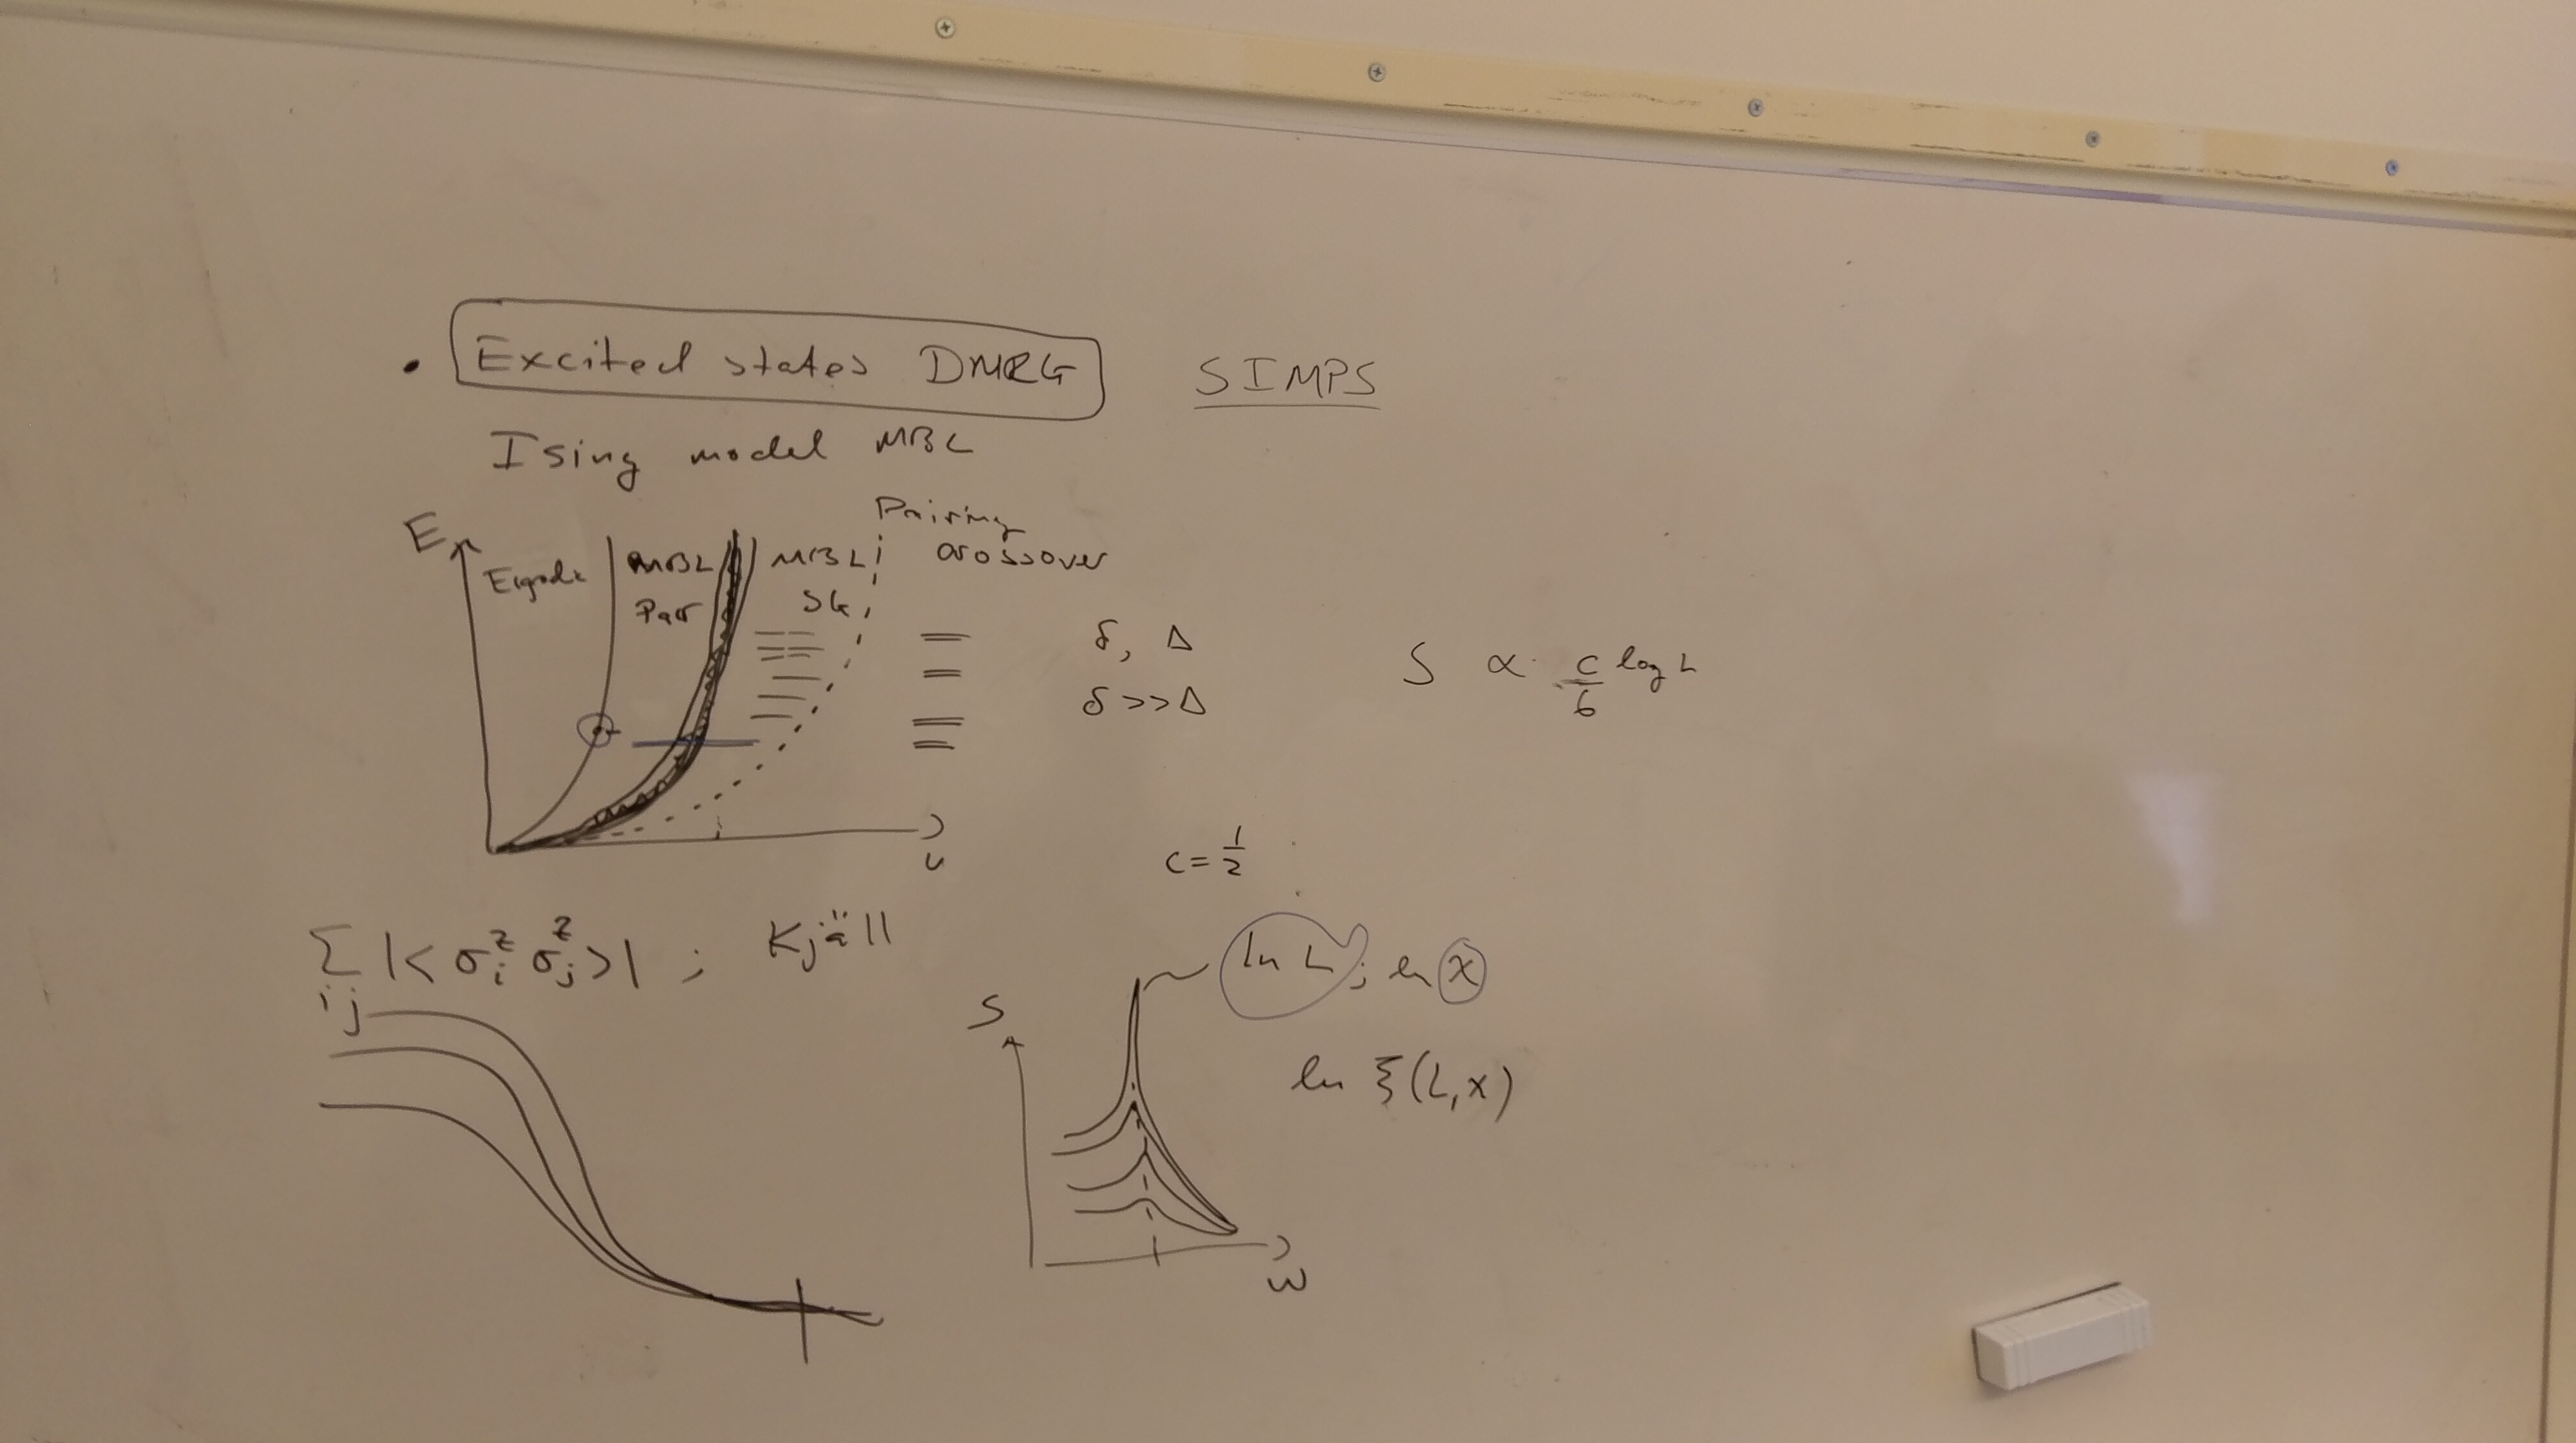
\includegraphics[width=0.9\textwidth, trim=12cm 2cm 40cm 12cm,clip]{figures/mblproject.jpg}

Other than that I continued the modularization, refactoring code. I'm trying to finish this as quickly as possible.

\end{markdown}

\section*{February}

\begin{markdown}
## Week 1
- Finished modularization. 
- Made another attempt to get Arpackc++ working to get eigenvalues of complex matrices. It worked! 
- Added the excited states module and started working on that.

## Week 2

- Changed the whole codebase to use complex numbers throughout. Having this double - complex switch is just messy, when complex numbers is ``lingua franca'' for MPS. 
- The xDMRG procedure is quite simple! Simply find all eigenvectors to the local effective hamiltonian,  i.e. $L-H-L$, where $H$ is an MPO, and chose the eigenvector with greatest overlap to the current state. Starting with a randomly oriented spin chain this converges usually to a highly excited state. Unfortunalely it doesn't let us target a specific energy, but perhaps if we use SIMPS in the beginning to target a specific part of the spectrum, we can then use xDMRG later to pinpoint a particular eigenstate in that region.

## Week 3

- To gauge how close the algorithm is to an eigenstate, I returned to the issue of computing the variance $\langle \Delta H \rangle = \langle H^2 \rangle - \langle H \rangle^2$. The method by C.West using characteristic functions seems very promising... if I could just get it to work. 

## Week 4

- Continued working on variances. 
- During the group meeting on Friday, a very fundamental error was pointed out to me. Essentially I hadn't been applying the unitary gates correctly; I applied them all, and then swapped. I am supposed to swap between every gate, and only then is a singla ``tebd'' step complete. It is amazing that I've gotten correct results all  this time despite this flaw. 


\end{markdown}
\section*{March}
\begin{markdown}
- The variance method by C.West works, almost. There is a discrepancy compared to the ``double MPO'' method I use for DMRG. Now I need to compute the variance using the regular method with the normal 2-site Hamiltonians. Turns out this is quite difficult, because the infinite number of crossterms need to be summed over. There are two places where this is described:

	- Zauner-Stauber, V., Vanderstraeten, L., Fishman, M. T., Verstraete, F., \& Haegeman, J. (2017). \href{https://doi.org/10.1103/PhysRevB.97.045145}{Variational optimization algorithms for uniform matrix product states} 
	
	- Vanderstraeten, L. (n.d.). \href{http://quantumtensor.pks.mpg.de/wp-content/uploads/2016/06/notes_2.pdf}{Tangent space methods for matrix product states}

- Later in March: Succeeded in computing the variance in three different ways.

	- The MPO-way, this is simply contracting two layers of Hamiltonian MPO's at each step instead of just one (as with the energy). Doing so gives $\langle H^2 \rangle$. For ``iDMRG`` we can of course subtract the current energy to the MPO. For instance in the Ising model, we subtract it from the term at the lowermost left corner: $g\sigma^x \rightarrow g\sigma^x - eI$, where $e$ is the per site energy and $I$ is an identity matrix of the appropriate size.
 	
 	- The ``Hamiltonian expansion'' way, where we simply compute $\mathrm{Var} H =  \langle (H - E)^2 \rangle $ directly. For the Ising model with nearest neighbor interactions this means that we get sums of 2-site terms squared, giving us an infinite number of cross-terms that have to be summed over or approximated assuming we are in the middle of an infinite chain. This turned out to be quite difficult, as the infinite sum -part was usually badly explained where I found it. 
 	
 	- The ``Characteristic function'' way where we get the moments of the distribution from derivatives of $\exp{(-iHt)}$. This method is almost identical to applying time evolution operators to the MPS, and similarly, one has to do a Suzuki-Trotter decomposition of the Hamiltonian and apply the operators in interleaved layers, just as in iTEBD. After applying all the layers, one computes the overlap with the non-evolved MPS. This technique had a couple of pitfalls that weren't mentioned. For instance, one has to allow the bond dimension to grow between when applying the layers, otherwise the results are very messy. Still, to avoid performance issues there needs to be an upper limit (say, 2-5 times larger than the current bond dimension), but it's not clear how to choose a good upper limit. 
 	
All three of these techniques are explained in detail in the DMRG++ document, and were presented towards the end of March in a Friday-fika meeting with the group.

Interestingly the two latter techniques are very costly computationally. The whole reason for doing them was to have ways of corroborating the size of the error given in the MPO-way. Essentially these three all agree very well, with one caveat being that in iDMRG-mode the MPO-method takes a while to converge because it remembers bad states far away at the edges of the system, whereas the other two always assume translation invariance. Note that the MPO-method also works with finite chains. Furthermore the MPO-method, which was expected to work poorly due to the scaling of the bond dimension, is in practice very fast.
	
\end{markdown}

\section*{April}
\begin{markdown}
- There are still a couple of unresolved issues with iDMRG, namely the delayed convergence. This problem has lingered almost since the beginning and I guess I never truly understood what Jens meant for me to do about it. Time to solve this.
	- The issue arises from the fact that 




- Started working on excited-state DMRG proper. There are a number of minor hurdles to address:

	- Full diagonalization of the effective Hamiltonian requires a lot of computing power. 

\end{markdown}


\section*{May}
\begin{markdown}

\end{markdown}

\section*{June}
\begin{markdown}
- Vacation by the end of June: Midsummer and trip to fjällen
\end{markdown}


\section*{July}
\begin{markdown}

\end{markdown}


\section*{August}
\begin{markdown}
- Looking at the \href{https://www.kth.se/student/kurser/org/SH}{course offering for PhD students}. There are several interesting courses, that I'll list here:
	- \href{https://www.kth.se/student/kurser/kurs/SI3200}{SI3200 Kondenserade materiens teori 7,5 hp} by Mats Wallin
	- \href{https://www.kth.se/student/kurser/kurs/SI3260}{SI3260 Kvanttransport 7,5 hp} by Jack Lidmar. It says the course is no longer available but perhaps one could ask nicely. 
	- \href{https://www.kth.se/student/kurser/kurs/LH3000}{LH3000 Basic Communication and Teaching 3.0 credits} by Mikael Cronhjort. I think this course is mandatory for teaching? I could be wrong.
	- \href{https://www.kth.se/student/kurser/kurs/SH3000}{SH3000 Bredd och etik i fysik 7,5 hp} by Pär Olsson. I think this course is mandatory for all PhD students. I already have 1/4 modules cleared. But I need to register properly.
	
	
	
- Some thoughts about courses: 
	- Perhaps Jens can ``make-up'' a reading course for me? I've heard that's something that has been done before. Perhaps then the topic may be even more relevant to my research or interests.
	- For SH3000, how do I register? Perhaps talk to Pär...
	- For LH3000, is this mandatory for teaching? Ask Pär...
	- \href{http://agenda.albanova.se/conferenceDisplay.py?confId=6537}{Introduction to High Performance Computing 7,5 hp} Registration for this summer school starts in April. 
	
- Looking at the study plan (eISP) I noticed that my courses counted from the master do not appear. Ask Pär about this? 

- Discussion with Loic on what to do with the excited states of the self-dual Ising model. First we discussed the following

	- I should check the sign of $J\_\mu$, make sure it's actually the correct one. 
	- It makes sense to have $\overline{\log J} = \log J\_\mu$ and similarly for $h\_\mu$.
	- The overlap threshold can be set somewhere below $\frac{1}{\sqrt{2}}$ in case that there are cat states. 
	- If the overlap threshold is not reached, how about making a full diag? What would happen then?
	- It might not be worthwile initializing the chain close to energy target first. A random chain will probably be close to the middle anyway.
	
	
	 Measure the following ($^\circ$ means $x,y,z$):
	 
	1. Average entanglement entropy S across the chain. Take the average over many realizations. Basically plot the average of S(l), where l is the position on the chain.
	2. $\frac{1}{L}|\langle \sigma^\circ \rangle|$ (or square instead of abs).
	3. $\langle\sigma\_i^\circ\sigma\_j^\circ \rangle$. This is the same as the one mentioned in Jens paper, i.e. the spin-glass observable. In the paper it is expressed as $\frac{1}{L} \sum\_{i,j} \langle n | \sigma\_i^\circ \sigma\_j^\circ | n \rangle $.
	4. $\frac{1}{L}\sum_{i,j} \langle  \sigma\_i^\circ \sigma\_j^\circ \rangle - \langle \sigma\_i^\circ \rangle \langle\sigma\_j^\circ \rangle $.
	5. Compute the single site density matrix in two ways according to the figure. Check that they are equivalent.
	\begin{figure}[h!]
		\centering
		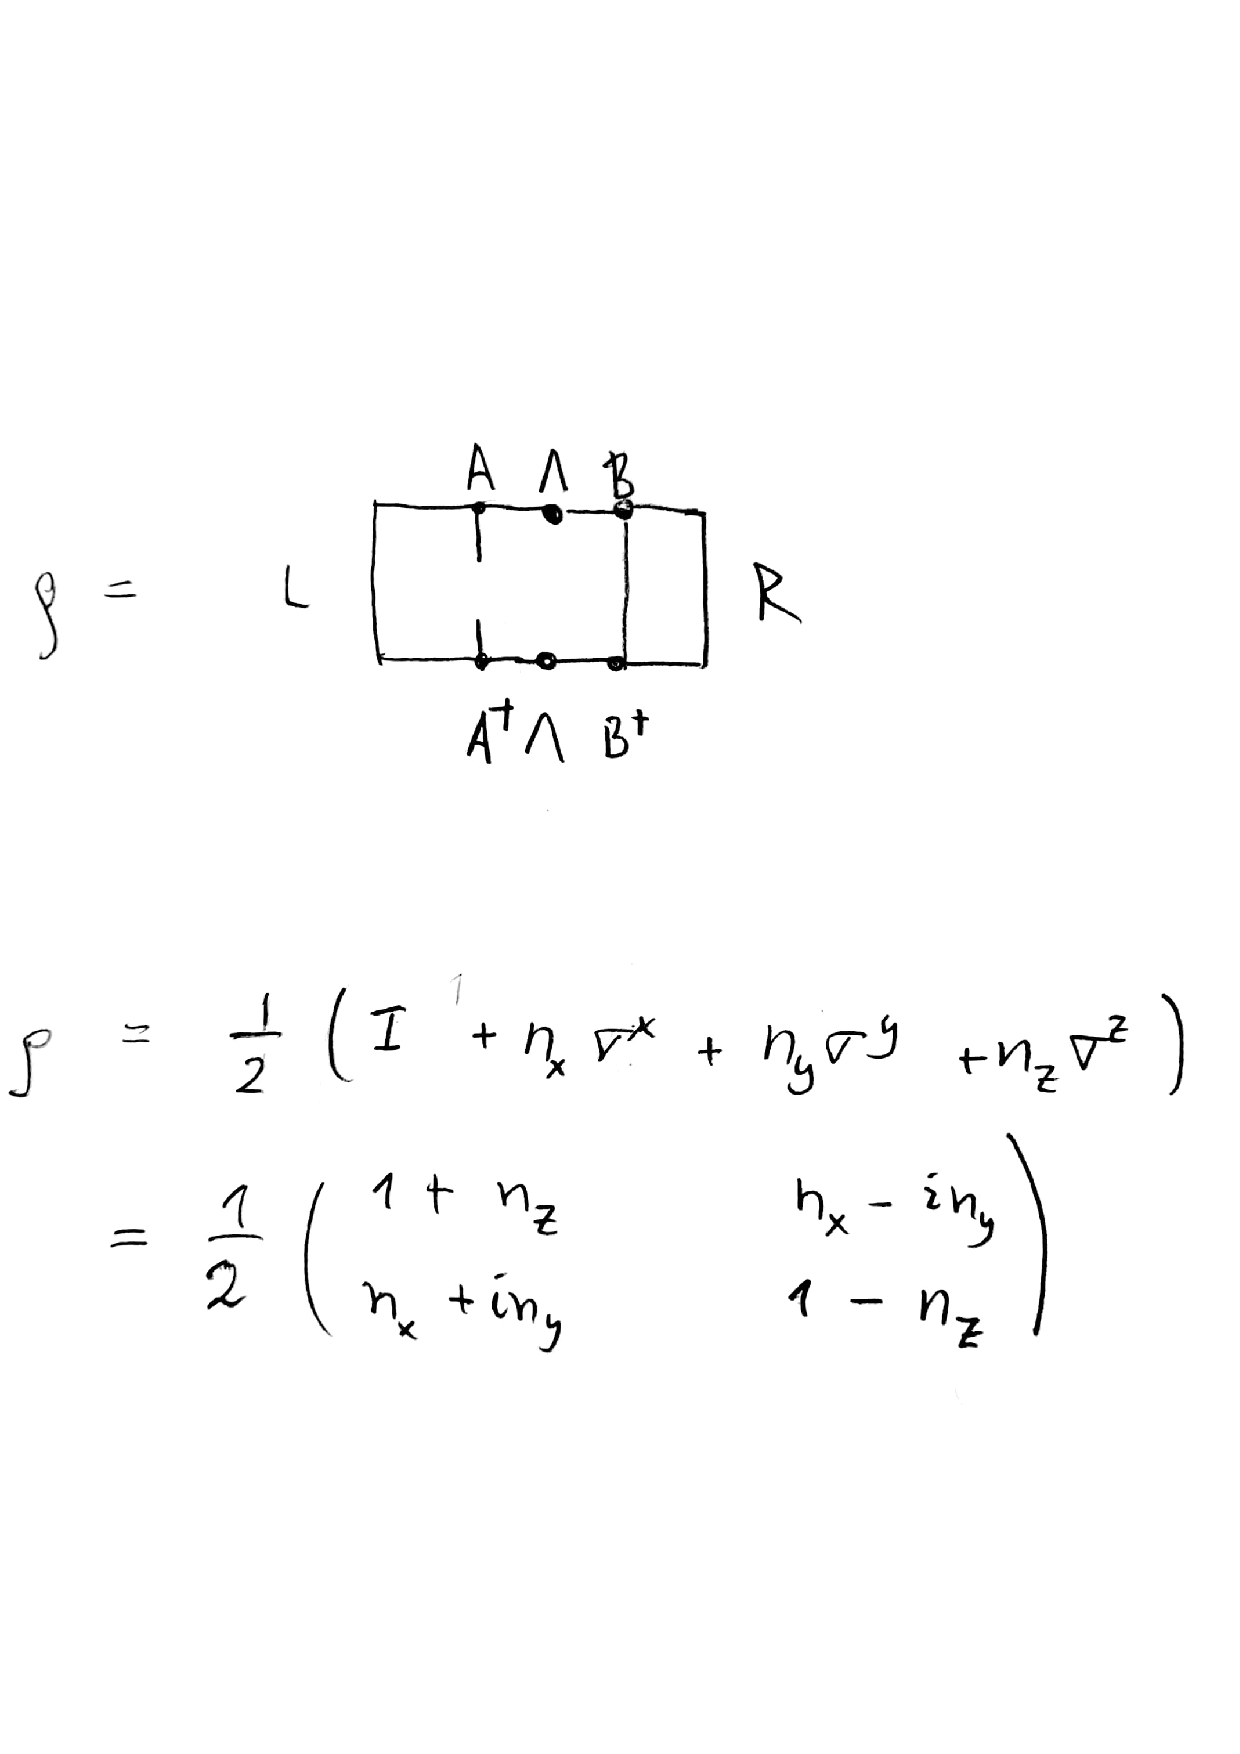
\includegraphics[width=0.6\textwidth]{figures/densitymatrix.pdf}
		\caption{The hermitian density matrix $\rho$ satisfies $\mathrm{Tr}(\rho) = 1$, the numbers $n\_x,n\_y,n\_z$ are real and $\mathrm{det}\rho = (1-|\mathbf{n}|^2)/4$. Since $\rho$ is positive we have $1\geq |\mathbf{n}|$. We can represent the density matrix $\rho$ by the vector $\mathbf{n}$, which lies in the unit ball. If $\rho$ is a pure state, its corresponding vector will lie on the surface of the sphere. Likewise if $|\mathbf{n}|=1$, then $\mathrm{Tr}(\rho) = 1$ and $\mathrm{det} \rho = 0$. This implies that one of the eigenvalues is zero and the other is one.}
	\end{figure}
		The eigenvalues $\lambda\_i$ of the density matrix $\rho$ can be used to compute the single-site entropy $S = -\sum\_i \lambda\_i \log \lambda\_i$.  Expectation values can be computed like $\langle \sigma^\circ \rangle = \mathrm{Tr}(\rho\sigma^\circ)$.

	- 
\end{markdown}

		

 













\end{document}